\documentclass[9pt]{beamer}

\usefonttheme{serif}
% \geometry{paperwidth=140mm,paperheight=105mm}

\RequirePackage[no-math]{fontspec}
\setmainfont{texgyretermes}[
  UprightFont = *-regular ,
  BoldFont = *-bold ,
  ItalicFont = *-italic ,
  BoldItalicFont = *-bolditalic ,
  Extension = .otf ,
  Scale = 1.0]
  
\setsansfont{texgyreheros}[
  UprightFont = *-regular ,
  BoldFont = *-bold ,
  ItalicFont = *-italic ,
  BoldItalicFont = *-bolditalic ,
  Extension = .otf ,
  Scale = 0.9]

\RequirePackage[UTF8,scheme=plain,fontset=none]{ctex}
\setCJKmainfont[BoldFont={FZHei-B01},ItalicFont={FZKai-Z03}]{FZShuSong-Z01}
\setCJKsansfont[BoldFont={FZHei-B01}]{FZKai-Z03}
\setCJKmonofont[BoldFont={FZHei-B01}]{FZFangSong-Z02}
\setCJKfamilyfont{zhsong}{FZShuSong-Z01}
\setCJKfamilyfont{zhhei}{FZHei-B01}
\setCJKfamilyfont{zhkai}[BoldFont={FZHei-B01}]{FZKai-Z03}
\setCJKfamilyfont{zhfs}[BoldFont={FZHei-B01}]{FZFangSong-Z02}
\newcommand*{\songti}{\CJKfamily{zhsong}}
\newcommand*{\heiti}{\CJKfamily{zhhei}}
\newcommand*{\kaishu}{\CJKfamily{zhkai}}
\newcommand*{\fangsong}{\CJKfamily{zhfs}}

\usepackage{anyfontsize}
\usepackage[english]{babel}
\usepackage{scrextend}
\addtokomafont{labelinglabel}{\normalfont\bfseries}
\usepackage{amsmath,amssymb}
\usepackage{bookmark}

\usetheme[sectionpage=none]{metropolis}
\setlength\abovecaptionskip{-1pt}
\setlength\belowcaptionskip{-1pt}
% adjust the space between caption and figure and table
% source: https://tex.stackexchange.com/questions/197879/how-to-adjust-spacing-between-caption-and-table-figure-in-beamer
\usefonttheme{professionalfonts}
\titlegraphic{
\includegraphics[width=1cm]{logo.png}}


\setbeamerfont{normal text}{family=\kaishu\sffamily}
\setbeamerfont{frametitle}{family=\large\bfseries\sffamily}
\setbeamerfont{title}{family=\bfseries}
\setbeamerfont{subtitle}{family=\kaishu}
\setbeamerfont{institute}{size=\small}
\definecolor{iron}{RGB}{0,82,67}
\setbeamercolor{frametitle}{bg=iron}
\setbeamercolor{progress bar}{fg=iron,bg=iron}


\setbeamertemplate{section in toc}[ball unnumbered]
\setbeamerfont{section in toc}{family=\heiti\sffamily}
\setbeamerfont{myTOC}{}
\AtBeginSection[]{\frame{\frametitle{目录}%
                  \usebeamerfont{myTOC}\tableofcontents[current]}}

\setcounter{tocdepth}{1}
\makeatletter
\setbeamertemplate{frametitle}[default][left,leftskip=\the\dimexpr\beamer@leftmargin-0.6cm\relax]
\makeatother


\setbeamertemplate{footline}
{%
   \leavevmode%
 \hskip1cm \fangsong \insertshortauthor \quad|\quad \insertshorttitle \hfill \normalfont  \insertframenumber\,/\,\inserttotalframenumber  \hskip1cm \hfill
   \vskip6pt%
}

\graphicspath{{image/}{figure/}{fig/}{img/}}
\usepackage{booktabs}
\usepackage{silence}
\WarningFilter{latexfont}{Font shape}
\let\scshape\relax
\usepackage{type1cm}
\AtBeginDocument{\usebeamerfont{normal text}}

\newcommand\email[1]{\href{mailto:#1}{\nolinkurl{#1}}}

\renewcommand\ttdefault{lmtt}

\author{ddswhu, syvshc, sikouhjw, osbertwang}
\title{Elegant\LaTeX{} 分享会}
\subtitle{模板使用初级入门}
\institute{ElegantLaTeX Program}
\date{2022/04/23}

\begin{document}

\maketitle


\begin{frame}\frametitle{目录}
\tableofcontents[hideallsubsections]
\end{frame}


\section{介绍}

\begin{frame}{关于 ElegantLaTeX}
Elegant\LaTeX{} 项目组由 \textcolor{iron}{ddswhu} 和\textcolor{iron}{小 L} 成立于 2012 年,致力于打造一系列美观、优雅、简便的模板方便用户使用。目前由 \href{https://github.com/ElegantLaTeX/ElegantNote}{ElegantNote},\href{https://github.com/ElegantLaTeX/ElegantBook}{ElegantBook},\href{https://github.com/ElegantLaTeX/ElegantPaper}{ElegantPaper} 组成,分别用于排版笔记,书籍和工作论文。

我们的联系方式如下,建议加入用户 QQ 群提问,这样能更快获得准确的反馈,加群时请备注 \LaTeX{} 或者 Elegant\LaTeX{} 相关内容。
\begin{itemize}
  \item 官网:\href{https://elegantlatex.org/}{https://elegantlatex.org/}
  \item GitHub 地址:\href{https://github.com/ElegantLaTeX/}{https://github.com/ElegantLaTeX/}
  \item Gitee 地址:\href{https://gitee.com/ElegantLaTeX}{https://gitee.com/ElegantLaTeX}
  \item CTAN 地址:\href{https://ctan.org/pkg/elegantbook}{https://ctan.org/pkg/elegantbook},note 和 paper 类似。
  \item 微博:Elegant\LaTeX{}
  \item 微信公众号:Elegant\LaTeX{}
  \item 用户 QQ 群:692108391
  \item 邮件:\email{elegantlatex2e@gmail.com}
\end{itemize}
\end{frame}

\begin{frame}{人员介绍}
  \begin{itemize}
    \item \textcolor{iron}{\bfseries 邓东升}:复旦大学经济学博士,又名 \underline{ddswhu}、\underline{EthanDeng},Elegant\LaTeX{} 的创立者和维护者。2010 年开始接触使用 \LaTeX{}。国内最早 Sublime Text 和 VS Code 推广者之一。\\[2ex]
    \item \textcolor{iron}{\bfseries 孙忠豪}:中科院数学与系统研究院硕士,又名\underline{乙醇},\underline{syvshc},Elegant\LaTeX{} 成员,HITBeamer 模板(哈工大)开发者和维护者,活跃在 QQ 用户群和 Github,校对翻译过 \TeX{} Live 包管理器的文档,热爱分享。\\[2ex]
    \item \textcolor{iron}{\bfseries 何骏炜}:广东工业大学硕士,又名\underline{死抠},\underline{sikouhjw},Elegant\LaTeX{} 成员,gdutthesis 开发者和维护者。自 2019 年开始在用户群群活跃,解答了 Github/知乎/LaTeXStudio.net/Stack Overflow 上诸多关于本模板的问题。\\[2ex]
    \item \textcolor{iron}{\bfseries 王然}:中国科学院大学博士后,又名\underline{啸行},\underline{ObsertWang}。目前负责维护 install-latex-guide-zh-cn 手册,曾参加过 Overleaf 公司 Advisor 项目,对多种编辑器、版本和 Overleaf 非常熟悉。
  \end{itemize}
\end{frame}


\begin{frame}{使用须知-适合}
  \begin{itemize}
    \item 对 \LaTeX{} 有一定了解,能够正常使用;
    \item 不习惯用默认的 article、book 文类;
    \item 文稿中有较多的数学公式;
    \item 接受模板的大部分设定;
    \item 认可模板的审美;
    \item 享受折腾。
  \end{itemize}  
\end{frame}


\begin{frame}{使用须知-不适合}
  \begin{itemize}
    \item 无法自行编译文档;
    \item 自定义想法很多;
    \item 具备单独写模板的能力;;
    \item 完全不想折腾,常年未更新过 TeX Live;
    \item CTeX 用户。
  \end{itemize}  
\end{frame}


% !TeX root = main.tex
\section{下载并安装 VSCode}
\begin{frame}[fragile]
  \frametitle{Windows 用户}
  \begin{itemize}[<+->]
    \item 在 VSCode 的官网 \href{https://code.visualstudio.com/}{https://code.visualstudio.com/} 选择 stable 版本进行下载
    \item 安装的时候注意将 ``通过 Code 打开'' 添加到上下文菜单:
  \end{itemize}
  \uncover<2>{
    \begin{center}
      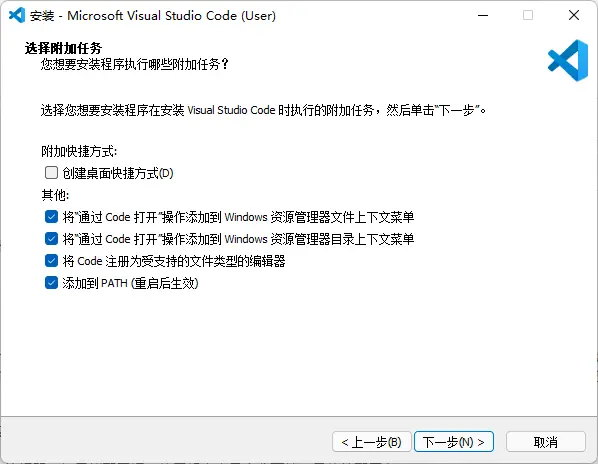
\includegraphics[width=8cm]{install-vs.png}
    \end{center}
  }
\end{frame}

\section{打开终端}

\begin{frame}[t]
  \frametitle{打开终端}
  \begin{description}[<+->]
    \item[WindowS 用户] 
    \begin{itemize}[<+->]
      \item \keys{\win + S} 后输入 ``cmd'' 并按下回车, 可以打开``命令提示符'', 也就是所谓的命令行, 或者使用 \keys{\ctrl + \shift + \enter} 来用管理员权限打开命令行.
      \only<2>{
        \begin{center}
          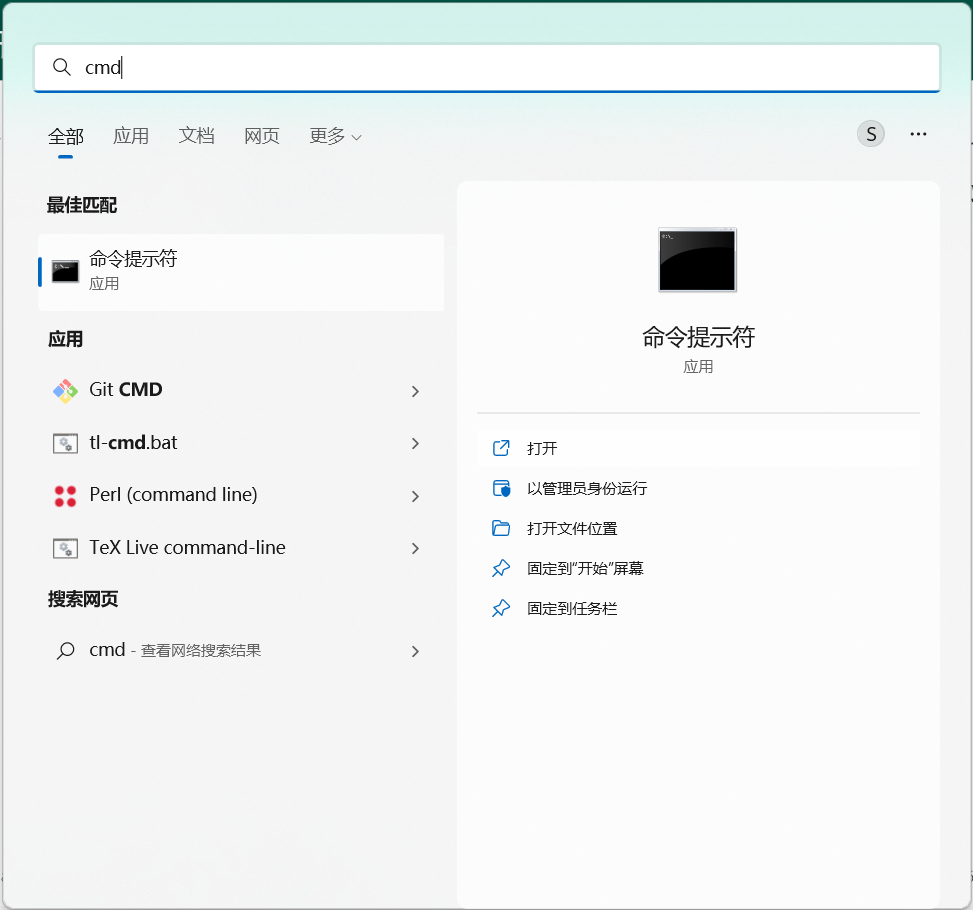
\includegraphics[width=6cm]{cmd.png}
        \end{center}
      }
      \item 在``文件资源管理器''的地址栏输入``cmd'' 并按下回车, 即可在当前位置打开命令行:
      \only<3>{
        \begin{center}
          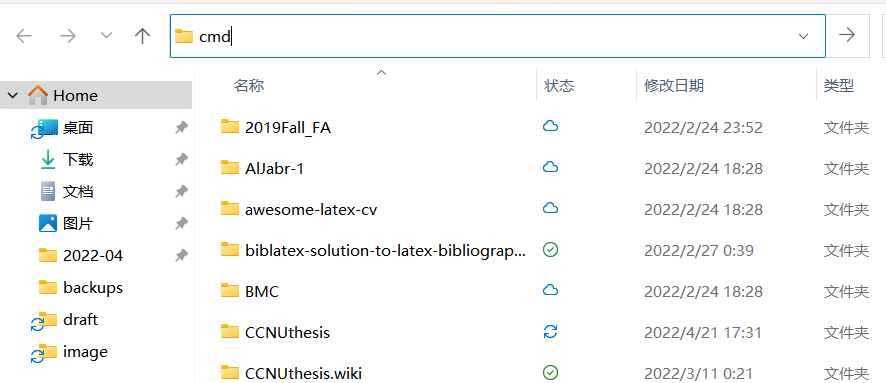
\includegraphics[width=7cm]{explorer.png}
        \end{center}
      }
      \item 如果安装了 Windows Terminal, 或者系统为 Win11, 可以在文件夹中或者文件夹上点击右键, 选择``在终端中打开'', 即可打开 Windows Terminal:
      \only<4>{
        \begin{center}
          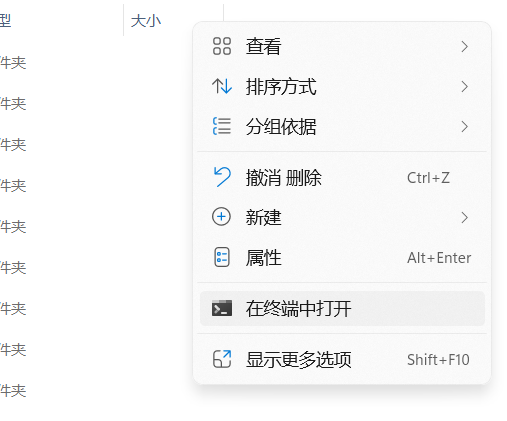
\includegraphics[width=5cm]{right-click.png}
        \end{center}
      }
    \end{itemize}
    \item[macOS 用户] \keys{\cmdmac + \SPACE} 后输入``terminal'', 即可打开终端. 
    \item[Linux 用户] \keys{\ctrl + \Alt + T} 即可打开终端. 
  \end{description}
  \uncover<7>{后面我们提到终端, 命令行均指这些东西, 并不做名字上的区分}
\end{frame}

\section{\texorpdfstring{\tlmgr}{tlmgr} 的使用}
\subsection{\texorpdfstring{\tlmgr}{tlmgr} 的简单介绍}
\begin{frame}[fragile]
  \frametitle{\tlmgr 的介绍}
  \begin{itemize}
    \item \tlmgr 是 \texlive 用来管理\emph{软件包}的工具;
    \item \emph{软件包}指的不只是可以通过 \lcmd{\usepackage} 调用的宏包, 而是所有 \texlive 包含的, 可以使用 \tlmgr 管理的内容, 比如平常所说的宏包, 如 \lstinline{amsmath.sty}, 一些说明文档, 如 \lstinline{lshort-zh-cn}, 一些可执行文件, 如 \lstinline{xetex.exe} 等等.
    \item \tlmgr 是 \textbf{T}eX\textbf{L}ive \textbf{M}ana\textbf{g}e\textbf{r} 的缩写;
    \item 命令行中运行 \cmd{tlmgr version} 就可以看到当前的\emph{修订版号}(revision), 通常输出如下
\begin{outputcode}
tlmgr revision 63033 (2022-04-15 07:19:42 +0200)
tlmgr using installation: C:/texlive/2022
TeX Live (https://tug.org/texlive) version 2022
\end{outputcode}
  \end{itemize}
\end{frame}

\subsection{\texorpdfstring{\tlmgr}{tlmgr} 的基本语法}

\begin{frame}[fragile]
  \frametitle{\tlmgr 的基本语法}
\begin{cmdcode}
tlmgr -global-options action -action-specific-options operand
\end{cmdcode}
\begin{enumerate}
  \item \cmd{-} 与 \cmd{--} 相同;
  \item 顺序不重要;
  \item \cmd{-dry-run}.
\end{enumerate}
\end{frame}

\subsection{更新软件包}

\begin{frame}[fragile,t]
  \frametitle{更新软件包 --- 操作: \frameaction{update}}
  \framesubtitle<1>{查看哪些软件包可以更新}
  \begin{onlyenv}<1>
\begin{cmdcode}
tlmgr update -list
\end{cmdcode}
\begin{outputcode}<1>
tlmgr.pl: package repository https://mirrors.tuna.tsinghua.edu.cn/CTAN/systems/texlive/tlnet (not verified: gpg unavailable)
tlmgr.pl: would save backups to C:/texlive/2022/tlpkg/backups
tlmgr.pl: skipping forcibly removed package: collection-texworks
update:   adjmulticol   [316k]: local:  62935, source:  63073
update:   hitex         [2565k]: local:  62529, source:  63073
update:   texlive-fr    [1394k]: local:  62853, source:  63071
update:   texlive-msg-translations [144k]: local:  63010, source:  63072
update:   texlive-scripts.win32 [36k]: local:  62199, source:  63068
update:   texlive-scripts [504k]: local:  63049, source:  63068
update:   utfsym         [4766k]: local:  56729, source:  63076
update:   xduts          [871k]: local:  63013, source:  63075
update:   zwpagelayout   [641k]: local:  53965, source:  63074  
\end{outputcode}
  \end{onlyenv}
  \framesubtitle<2>{更新全部软件包}
  \begin{onlyenv}<2>
\begin{cmdcode}
tlmgr update -self -all
\end{cmdcode}
\begin{outputcode}
tlmgr.pl: package repository https://mirrors.tuna.tsinghua.edu.cn/CTAN/systems/texlive/tlnet (not verified: gpg unavailable)
tlmgr.pl: saving backups to C:/texlive/2022/tlpkg/backups
tlmgr.pl: no self-updates for tlmgr available
[ 1/16, ??:??/??:??] update: babel-french [567k] (59997 -> 63088) ... done
[ 2/16, 00:02/01:48] update: l3backend [894k] (63025 -> 63089) ... done
...
[16/16, 01:23/01:23] update: collection-luatex [1k] (62829 -> 63081) ... done
running mktexlsr ...
done running mktexlsr.
running mtxrun --generate ...
done running mtxrun --generate.
running updmap-sys ...
...
tlmgr.pl: package log updated: C:/texlive/2022/texmf-var/web2c/tlmgr.log
tlmgr.pl: command log updated: C:/texlive/2022/texmf-var/web2c/tlmgr-commands.log
\end{outputcode}
  \end{onlyenv}
  \framesubtitle<3>{其他的功能}
  \begin{enumerate}[<3->]
    \item 更新软件包 \pkg{pkg1}, \pkg{pkg2}:
\begin{cmdcode}
tlmgr update pkg1 pkg2
\end{cmdcode}
    \item 如果更新全部宏包时不想更新 \pkg{pkg1}, \pkg{pkg2}:
\begin{cmdcode}
tlmgr update -self -all -exclude pkg1 -exclude pkg2
\end{cmdcode}
    \item 如果更新过程被中断
\begin{cmdcode}
tlmgr update -self -all -reinstall-forcibly-removed
\end{cmdcode}
  \end{enumerate}
\end{frame}

\subsection{查看软件包信息}

\begin{frame}[fragile]
  \frametitle{查看软件包信息 --- 操作: \frameaction{info}}
  \framesubtitle<1>{列出软件包的详细信息}

  \begin{onlyenv}<1>
\begin{cmdcode}
tlmgr info pkg1 pkg2
\end{cmdcode}
\begin{outputcode}
package:     ctex
category:    Package
shortdesc:   LaTeX classes and packages for Chinese typesetting
longdesc:    ctex is a collection of macro packages and document classes for LaTeX Chinese typesetting.
installed:   Yes
revision:    61285
sizes:       src: 481k, doc: 1137k, run: 1753k
relocatable: No
cat-version: 2.5.8
cat-license: lppl1.3c
cat-topics:  chinese book-pub class
cat-contact-bugs: https://github.com/CTeX-org/ctex-kit/issues
cat-contact-support: https://github.com/CTeX-org/ctex-kit/issues
cat-contact-repository: https://github.com/CTeX-org/ctex-kit
cat-contact-home: http://www.ctex.org/HomePage
collection:  collection-langchinese
\end{outputcode}
  \end{onlyenv}

  \framesubtitle<2>{查看软件包的文件信息}
  \begin{onlyenv}<2>
\begin{cmdcode}
tlmgr info -list pkg1 pkg2
\end{cmdcode}
\begin{outputcode}
# 省略 tlmgr info tabularray 的内容 #
Included files, by type:
run files:
texmf-dist/tex/latex/tabularray/tabularray-2021.sty
texmf-dist/tex/latex/tabularray/tabularray.sty
doc files:
texmf-dist/doc/latex/tabularray/README.txt details="Readme"
texmf-dist/doc/latex/tabularray/tabularray.pdf details="Package documentation"
texmf-dist/doc/latex/tabularray/tabularray.tex  
\end{outputcode}
  \end{onlyenv}
\end{frame}

\subsection{回滚软件包的版本}

\begin{frame}[fragile]
  \frametitle{回滚软件包的版本 --- 操作: \frameaction{restore}}
  
  \framesubtitle<1>{查看某个软件包的备份} 
  % \begin{onlyenv}<1>
\begin{cmdcode}
tlmgr restore pkg
\end{cmdcode}
\begin{outputcode}
tlmgr restore functional
Available backups for functional: 62926 (2022-04-17 11:15)
\end{outputcode}
  % \end{onlyenv}
  \framesubtitle<2>{将某个软件包回滚为备份}

\begin{uncoverenv}<2>
\begin{cmdcode}
tlmgr restore pkg revision
\end{cmdcode}
\begin{outputcode}
tlmgr restore functional 62926
Do you really want to restore functional to revision 62926 (y/N): y
Restoring functional, 62926 from C:/texlive/2022/tlpkg/backups/functional.r62926.tar.xz
running mktexlsr ...
done running mktexlsr.
running mtxrun --generate ...
done running mtxrun --generate.
tlmgr.pl: package log updated: C:/texlive/2022/texmf-var/web2c/tlmgr.log
tlmgr.pl: command log updated: C:/texlive/2022/texmf-var/web2c/tlmgr-commands.log
\end{outputcode}
\end{uncoverenv}
\end{frame}

\subsection{修改 \texorpdfstring{\tlmgr}{tlmgr} 的设置}

\begin{frame}[fragile]
  \frametitle{修改 \tlmgr 的设置 --- 操作: \frameaction{option}}
  \framesubtitle{设置软件包的更新源}
\begin{cmdcode}
tlmgr option repository mirror
\end{cmdcode}
\uncover<2>{值得一提: \cmd{repository} = \cmd{repo}}
\end{frame}

\subsection{更多内容}

\begin{frame}
  \frametitle{更多内容}
  如果想了解更多关于 tlmgr 的信息, 欢迎阅读我翻译的 \href{http://mirrors.ctan.org/info/tlmgr-intro-zh-cn/tlmgr-intro-zh-cn.pdf}{tlmgr-intro-zh-cn} 以及 \href{https://www.tug.org/texlive/doc/tlmgr.html}{tlmgr 的官方文档}
\end{frame}

\section{命令行编译}

\subsection{简单配置一下 VSCode}

\begin{frame}
  \frametitle{简单配置一下 VSCode}
  \begin{enumerate}[<+->]
    \item 更改语言为中文
    \item 安装 LaTeX Workshop (LW)
  \end{enumerate}
\end{frame}

\subsection{命令行操作}

\begin{frame}[fragile]
  \frametitle{命令行操作}
  \begin{enumerate}[<+->]
    \item \cmd{cd};
    \item \cmd{dir} (Windows), \cmd{ls} (Linux, macOS);
    \item \cmd{mkdir};
    \item \cmd{del} (Windos), \cmd{rm} (Linux, macOS);
    \item \cmd{move} (Windos), \cmd{mv} (Linux, macOS);
    \item \cmd{copy} (Windos), \cmd{cp} (Linux, macOS);
    \item \cmd{code}
  \end{enumerate}
\end{frame}

\subsection{使用命令行编译 \LaTeX 文件}
\subsubsection{第一次编译}

\begin{frame}[fragile]
  \frametitle{使用命令行编译 \LaTeX 文件}
  \framesubtitle{第一次编译}
\begin{onlyenv}<1,2>
  \begin{enumerate}[<+->]
    \item 在 \directory{D:/folder} 文件夹下新建 \directory{main.tex}, 输入以下内容
\begin{latexcode}
\documentclass{article}
\begin{document}
  Hello \LaTeX!
\end{document}  
\end{latexcode}
    \item 在命令行中运行 
\begin{cmdcode}
pdflatex main.tex
\end{cmdcode}
\begin{outputcode}
This is pdfTeX, Version 3.141592653-2.6-1.40.24 (TeX Live 2022) (preloaded format=pdflatex)
restricted \write18 enabled.
entering extended mode
(./main.tex
LaTeX2e <2021-11-15> patch level 1
L3 programming layer <2022-02-24>
(/home/syvshclily/texlive/2022/texmf-dist/tex/latex/base/article.cls
Document Class: article 2021/10/04 v1.4n Standard LaTeX document class
(/home/syvshclily/texlive/2022/texmf-dist/tex/latex/base/size10.clo))
(/home/syvshclily/texlive/2022/texmf-dist/tex/latex/l3backend/l3backend-pdftex.
def) (./main.aux) [1{/home/syvshclily/texlive/2022/texmf-var/fonts/map/pdftex/u
pdmap/pdftex.map}] (./main.aux) )</home/syvshclily/texlive/2022/texmf-dist/font
s/type1/public/amsfonts/cm/cmr10.pfb>
Output written on main.pdf (1 page, 12962 bytes).
Transcript written on main.log. 
\end{outputcode}
  \end{enumerate}  
\end{onlyenv}
\begin{onlyenv}<3>
  \begin{itemize}
    \item \directory{main.aux}: 辅助文件;
    \item \directory{main.log}: 日志文件;
    \item \directory{main.pdf}: 输出的 PDF 文件.
  \end{itemize}
\end{onlyenv}
\end{frame}

\subsubsection{遇到错误}

\begin{frame}[fragile]
  \frametitle{使用命令行编译 \LaTeX 文件}
  \framesubtitle{遇到错误}
\begin{onlyenv}<1-2>
  \begin{enumerate}[<+->]
    \item \lcmd{\LaTeX} $ \Rightarrow $ \lcmd{\LaTex}
    \item 在命令行中运行
\begin{cmdcode}
pdflatex main.tex
\end{cmdcode}
\begin{outputcode}
This is pdfTeX, Version 3.141592653-2.6-1.40.24 (TeX Live 2022) (preloaded format=pdflatex)
restricted \write18 enabled.
entering extended mode
(./main.tex
LaTeX2e <2021-11-15> patch level 1
L3 programming layer <2022-02-24>
(/home/syvshclily/texlive/2022/texmf-dist/tex/latex/base/article.cls
Document Class: article 2021/10/04 v1.4n Standard LaTeX document class
(/home/syvshclily/texlive/2022/texmf-dist/tex/latex/base/size10.clo))
(/home/syvshclily/texlive/2022/texmf-dist/tex/latex/l3backend/l3backend-pdftex.
def) (./main.aux)
! Undefined control sequence.
l.3   Hello \Latex
                  !
?  
\end{outputcode}
  \end{enumerate}  
\end{onlyenv}
\begin{onlyenv}<3>
  \begin{itemize}
    \item \keys{I + <cs> + \enter};
    \item \keys{X + \enter};
    \item \keys{H + \enter}.
  \end{itemize}
\end{onlyenv}
\end{frame}

\subsubsection{编译选项}

\begin{frame}[fragile]
  \frametitle{使用命令行编译 \LaTeX 文件}
  \framesubtitle{编译选项}

\begin{cmdcode}
pdflatex --option1 --option2=<string> main.tex
\end{cmdcode}
  
\begin{enumerate}[<+->]
  \item \cmd{--halt-on-error}
  \item \cmd{--interactionmode=<errorstop|scroll|batch|nonstop>mode}
  \item \cmd{--synctex=1}
  \item \cmd{--jobname=<string>}
  \item \cmd{--output-directory=<string>}
  \item \cmd{--shell-escape}
\end{enumerate}
\end{frame}

\subsubsection{多次编译}

\begin{frame}[fragile,t]
  \frametitle{使用命令行编译 \LaTeX 文件}
  \framesubtitle{目录与交叉引用}
\begin{latexcode}
% main.tex
\documentclass{article}
\begin{document}
\tableofcontents
\section{One}\label{sec:one}
  We are in section \ref{sec:one}
\end{document}
\end{latexcode}
\only<2>{
  \begin{center}
    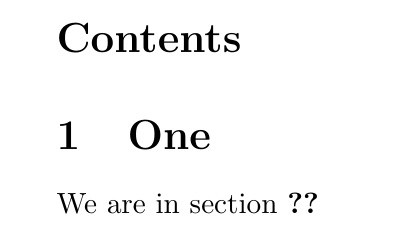
\includegraphics[height=3cm]{cross-ref.png}
  \end{center}
}
\begin{onlyenv}<3>
\begin{latexcode}
% main.aux
\relax 
\@writefile{toc}{\contentsline {section}{\numberline {1}One}{1}{}\protected@file@percent }
\newlabel{sec:one}{{1}{1}}
\gdef \@abspage@last{1}
% main.toc
\contentsline {section}{\numberline {1}One}{1}{}%
\end{latexcode}  
\end{onlyenv}
\only<4>{
  \begin{center}
    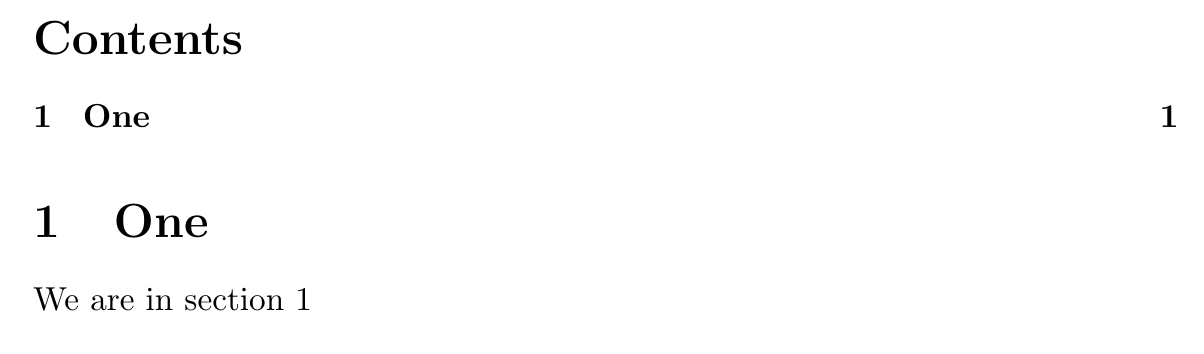
\includegraphics[height=3cm]{cross-ref-right.png}
  \end{center}
}
\end{frame}

\subsubsection{参考文献}

\begin{frame}[fragile, t]
  \frametitle{使用命令行编译 \LaTeX 文件}
  \framesubtitle{参考文献}

\begin{latexcode}
\documentclass{article}
\begin{document}
  text\cite{article-full}
  \bibliographystyle{plain}
  \bibliography{xampl.bib}
\end{document}
\end{latexcode}

\begin{onlyenv}<2>
\begin{cmdcode}
pdflatex main.tex
bibtex main.aux
pdflatex main.tex
pdflatex main.tex
\end{cmdcode}  
\end{onlyenv}

\begin{onlyenv}<3>
  \begin{center}
    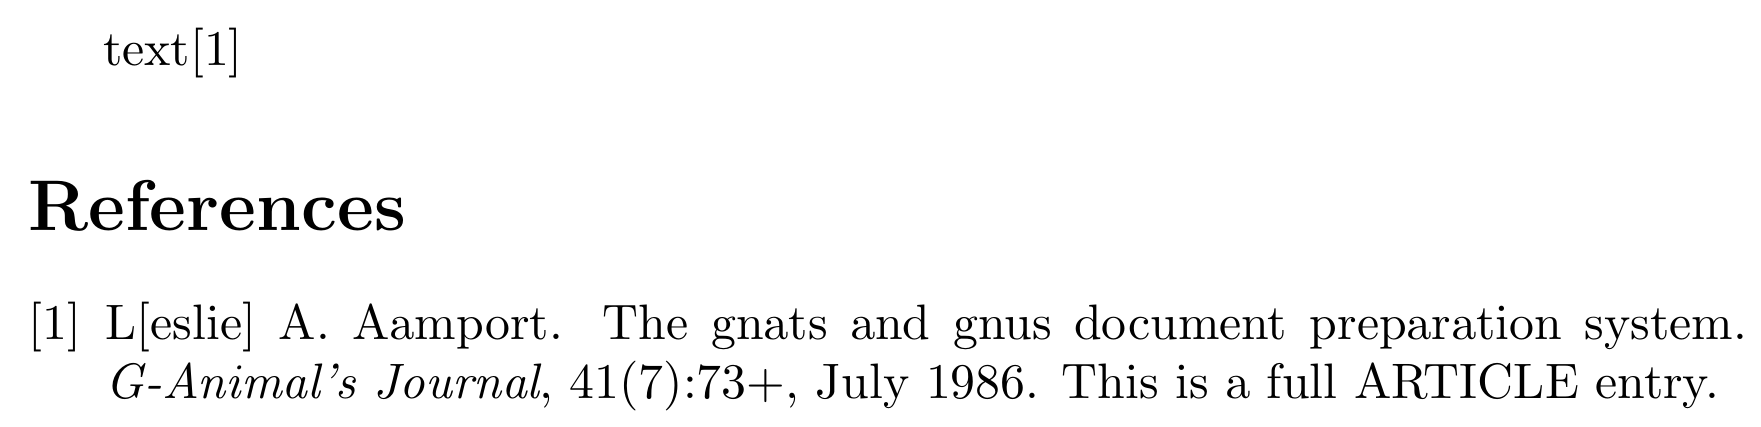
\includegraphics[width=\textwidth]{bib-ref.png}
  \end{center}
\end{onlyenv}
\end{frame}

\subsubsection{更强大的工具: \texttt{latexmk}}

\begin{frame}[fragile, t]
  \frametitle{使用命令行编译 \LaTeX 文件}
  \framesubtitle{更强大的工具: \texttt{latexmk}}

\begin{latexcode}
% main.tex
\documentclass{article}
\begin{document}
\tableofcontents
\section{One}\label{sec:one}
  We are in section \ref{sec:one}, 
  and we have a cite \cite{article-full}
  \bibliographystyle{plain}
  \bibliography{xampl.bib}
\end{document}
\end{latexcode}

\begin{cmdcode}
latexmk -pdf main.tex
\end{cmdcode}
\end{frame}

\subsubsection{更多}

\begin{frame}
  \frametitle{使用命令行编译 \LaTeX 文件}
  \framesubtitle{更多的内容}
  更多内容可以参见
  \begin{itemize}
    \item \texttt{\textbf{texdoc} latexmk}
    \item \cmd{pdflatex --help}
    \item \href{https://syvshc.github.io/2022-03-06-latex-terminal-compiling/}{在终端中编译 \LaTeX}
  \end{itemize}
\end{frame}

\section{安装外部宏包}
\subsection{检查宏包是否安装}

\begin{frame}[fragile]
  \frametitle{安装外部宏包}
  \framesubtitle{检查一个宏包是否被安装了}
\begin{cmdcode}
tlmgr info pkg
# or 
kpsewhich pkg.sty
\end{cmdcode}
\end{frame}

\begin{frame}[fragile, t]
  \frametitle{安装外部宏包}
  \framesubtitle{手动安装宏包}
\begin{onlyenv}<1>
\begin{latexcode}
% mypackage.sty
\NeedsTeXFormat{LaTeX2e}[2017/04/15]
\ProvidesPackage{mypackage}[2022/4/20 v1.0 test]
\newcommand{\mycmd}{Hello \LaTeX}  
\end{latexcode}
\end{onlyenv}
\begin{onlyenv}<2->
  \begin{enumerate}
    \item 在 \directory{C:/texlive/texmf-local/tex/latex} 文件夹下新建文件夹 \directory{mypackage};
    \item 将 \texttt{mypackage.sty} 放进去;
    \item 命令行运行 \cmd{texhash}.
  \begin{outputcode}
  texhash: Updating C:/texlive/texmf-local/ls-R...
  texhash: Updated C:/texlive/texmf-local/ls-R.
  texhash: Updating C:/texlive/2022/texmf-config/ls-R...
  texhash: Updated C:/texlive/2022/texmf-config/ls-R.
  texhash: Updating C:/texlive/2022/texmf-var/ls-R...
  texhash: Updated C:/texlive/2022/texmf-var/ls-R.
  texhash: Updating C:/texlive/2022/texmf-dist/ls-R...
  texhash: Updated C:/texlive/2022/texmf-dist/ls-R.
  texhash: Done.
  \end{outputcode}
  \end{enumerate}
\end{onlyenv}
\begin{onlyenv}<1, 3>
\begin{latexcode}
% main.tex
\documentclass{article}
\usepackage{mypackage}
\begin{document}
  \mycmd
\end{document}
\end{latexcode}
\end{onlyenv}
\end{frame}

\section{配置 VSCode 的编译链}

\begin{frame}
  \frametitle{配置 VSCode 的编译链}
  由于内容中演示居多, 这里只给出一个 \href{https://gitee.com/xkwxdyy/CCNUthesis/wikis/\%E5\%B8\%B8\%E8\%A7\%81\%E9\%97\%AE\%E9\%A2\%98FAQ/\%E5\%A6\%82\%E4\%BD\%95\%E5\%AE\%89\%E8\%A3\%85\%E3\%80\%81\%E9\%85\%8D\%E7\%BD\%AE\%E5\%92\%8C\%E4\%BD\%BF\%E7\%94\%A8VScode\#config-LW}{Wiki}. 
\end{frame}
% !TeX root = main.tex

\section{模板是什么}
\begin{frame}{发行版与模板}
  发行版与模板的关系是什么?\pause

  首先我们要明确什么是发行版和模板。\pause

  发行版:一个 \TeX 发行版是 \TeX 排版引擎、支持排版的文件(基本格式、\LaTeX 宏包、字体等)以
  及一些辅助工具的集合。\pause

  模板:模板本质上是一份实现特定目的、效果的代码,呈现形式一般为 cls(文档类)或者 sty(宏包)。模板具有以下特性:
  \begin{itemize}
    \item 模板维护者需要撰写专门的文档和例子;
    \item 普通用户应该能在阅读模板的使用说明后,较为自主地使用该模板;
    \item 即使是模板,也只为「100\% 使用预定义样式」的使用场景提供便利。
  \end{itemize}
\end{frame}

\begin{frame}[fragile]{模板是如何下载到你本地发行版的}
  模板到你本地发行版里,有几个过程:
  \begin{enumerate}
    \item 将发行版上传给 CTAN;
    \item 被发行版收录(如 TeX Live);
    \item 发行版镜像源更新;
    \item 用包管理器安装或升级。
  \end{enumerate}

  也就是说,发行版里其实安装了很多模板。
  
  ElegantLaTeX 的模板在 TeX Live 2019 之后就收录进 TeX Live 里了,也就是说,如果你的发行版在 TeX Live 2019 之后,那么你本地发行版就是有模板的。

  可以通过 \lstinline{kpsewhich elegantbook.cls}、\lstinline{texdoc -l elegantbook} 找到模板文件。
\end{frame}

\begin{frame}{那为什么还要下载最新版?}
  模板是有很多版本的,一般来说是通过更新全部宏包来获取最新版模板。

  在需要模板某些新功能的时候,也可以手动下载最新版模板,解压后使用。
\end{frame}

\section{模板基本使用}
\begin{frame}{如何编译模板}
  用 xelatex 编译。
\end{frame}

\begin{frame}[fragile]{模板手册}
  命令行输入 \lstinline{texdoc elegantbook}。
\end{frame}

\begin{frame}{模板基础设置}
  \begin{itemize}
    \item 中文字体
    \item 数学字体
    \item 参考文献
  \end{itemize}
\end{frame}

\begin{frame}{安装方正字体}
  
\end{frame}

\begin{frame}[fragile]{字体相关命令}
  \lstinline{fc-cache}、\lstinline{fc-list}。
\end{frame}

\begin{frame}[standout]
  Thank you!
\end{frame}

\end{document}

